\documentclass[fleqn]{jsarticle}

\usepackage{graphicx}
\usepackage{amsmath,amssymb}
\usepackage{amsmath}
\usepackage{fancyhdr}

\pagestyle{fancy}
\fancyhead[RE,RO]{先端データ解析論 レポート}

\usepackage{xcolor}
\usepackage[justification=centering]{caption}
\usepackage{listings}
\renewcommand{\lstlistingname}{リスト}
\lstset{language=Python,%
        % basicstyle=\footnotesize,%
        basicstyle=\tiny,%
        commentstyle=\textit,%
        classoffset=1,%
        keywordstyle=\bfseries,%
      	frame=tRBl,framesep=5pt,%
      	showstringspaces=false,%
        linewidth=38em,
      	}%

\begin{document}

\newcommand{\argmax}{\mathop{\rm argmax}\limits}
\newcommand{\argmin}{\mathop{\rm argmin}\limits}

\title{先端データ解析論 第5回レポート}
\author{電子情報学専攻 48-176403 石毛真修}
\maketitle



\section*{大問1.}
相補条件
\begin{eqnarray}
  \alpha_i (y_i {\mathbf \omega^{\mathrm T} {\mathbf x}_i - 1 + \xi_i}) = 0\\
  \beta_i \xi_i = 0
\end{eqnarray}
より,次が成り立つことを示す.

\begin{eqnarray}
  \alpha_i = 0 \to y_i {\mathbf \omega}^{\mathrm T} {\mathbf x}_i \geq 1\\
  0 < \alpha_i < C \to y_i {\mathbf \omega}^{\mathrm T} {\mathbf x}_i = 1\\
  \alpha_i = C \to y_i {\mathbf \omega}^{\mathrm T} {\mathbf x}_i \leq 1\\
  y_i {\mathbf \omega}^{\mathrm T} {\mathbf x}_i > 1 \to \alpha_i = 0\\
  y_i {\mathbf \omega}^{\mathrm T} {\mathbf x}_i < 1 \to \alpha_i = C
\end{eqnarray}


\subsection*{証明}
\subsubsection*{(3)}
$\alpha_i + \beta_i = C$ より,$\beta_i = C$.\\
式(2)より,$\beta_i \neq 0$なので,$\xi_i = 0$.\\
よって,$y_i {\mathbf \omega}^{\mathrm T} {\mathbf x}_i - 1 + \xi_i \geq 0$なので,
$y_i {\mathbf \omega}^{\mathrm T} {\mathbf x}_i \geq 1$

\subsubsection*{(4)}
$\alpha_i + \beta_i = C$ より,$\beta_i \neq 0$.
これと式(2)より,$\xi_i = 0$.\\
また,$\alpha_i \neq 0$ であるので,式(1)より
$y_i {\mathbf \omega}^{\mathrm T} {\mathbf x}_i - 1 + \xi_i = 0$.\\
以上から,$y_i {\mathbf \omega}^{\mathrm T} {\mathbf x}_i = 1$

\subsubsection*{(5)}
式(1)より,$\alpha_i \neq 0$なので,
$y_i {\mathbf \omega}^{\mathrm T} {\mathbf x}_i - 1 + \xi_i = 0$.\\
$\xi_i \geq 0$であるので,
$y_i {\mathbf \omega}^{\mathrm T} {\mathbf x}_i \leq 1$

\subsubsection*{(6)}
$y_i {\mathbf \omega}^{\mathrm T} {\mathbf x}_i - 1 > 0$なので,
$y_i {\mathbf \omega}^{\mathrm T} {\mathbf x}_i - 1 + \xi_i > \xi_i \geq 0$.\\
よって,$y_i {\mathbf \omega}^{\mathrm T} {\mathbf x}_i - 1 + \xi_i > 0$であり,
式(1)より,$\alpha_i = 0$.

\subsubsection*{(7)}
$y_i {\mathbf \omega}^{\mathrm T} {\mathbf x}_i - 1 <  0$であるので,
$0 \leq y_i {\mathbf \omega}^{\mathrm T} {\mathbf x}_i - 1 + \xi_i < \xi_i$.
よって,$\xi_i > 0$.\\
これと式(2)より,$\beta_i = 0$.
$\alpha_i + \beta_i = C$なので,$\alpha_i = C$.


\newpage

\section*{大問2.}
線形モデル
$f_{{\mathbf \omega}, b}(\mathbf x) = {\mathbf \omega}^{\mathrm T} {\mathbf + b}$
に対するSVMの劣勾配アルゴリズムを実装する.

\begin{center}
\begin{tabular}{c}
  \begin{lstlisting}[]
    import numpy as np
    import matplotlib.pyplot as plt
    import matplotlib

    # Generate data to fit
    rs = np.random.RandomState(42)
    n = 200
    X = np.array([np.concatenate((rs.randn(n//2) + 5, rs.randn(n//2) - 5)),
                            rs.randn(n)])
    Y = np.concatenate((np.ones(n//2), - np.ones(n//2)))
    Y[:3] = -1
    Y[n//2:n//2 + 3] = 1
    X[1, :3] += 5
    X[1, n//2:n//2 + 3] -= 5

    # Fitting
    p_rs = np.random.RandomState(15)
    theta = np.zeros(n)
    b = 0

    def f_th(x):
        global theta, b, X
        return x @ X @ theta + b

    def sub_diff(i, k):
        """Sub-differentiate by k_th theta"""
        global theta, b, X, y
        if 1 - y[i] * f_th(X[:, i]) > 0:
            return - y[i] * np.matmul(X[:, k], X[:, i])
        else:
            return 0

    def sub_diff_b(i):
        """Sub-differentiate by b"""
        global theta, b, X, y
        if 1 - y[i] * f_th(X[:, i]) > 0:
            return - y[i]
        else:
            return 0

    def update_theta(k, lamb=0.01):
        """Return update for k_th theta"""
        global theta, n
        val = lamb * theta[k]
        for i in range(n):
            val += sub_diff(i, k)
        return val

    def update_b():
        """Return update for b"""
        global n
        val = 0
        for i in range(n):
            val += sub_diff_b(i)
        return val

    iter_num = 200
    for l in range(iter_num):
        eps = 0.1
        new_theta = np.copy(theta)
        for i, t in enumerate(theta):
            new_theta[i] -= eps * update_theta(i)
        b -= eps * update_b()
        theta = new_theta

    w = X @ theta
    print(w)

    # Show result
    plt.scatter(X[0, np.where(Y==1)], X[1, np.where(Y==1)], c='r', marker='x')
    plt.scatter(X[0, np.where(Y==-1)], X[1, np.where(Y==-1)], c='b', marker='o')
    _x = np.linspace(-10, 10)
    plt.plot(_x, b - _x * w[0] / w[1])
    plt.ylim(-10, 10)
    plt.xlim(-10, 10)
    plt.show()

  \end{lstlisting}
\end{tabular}{c}
\end{center}

このコードを実行すると次のような結果を得た.
\begin{figure}[h]
  \begin{center}
    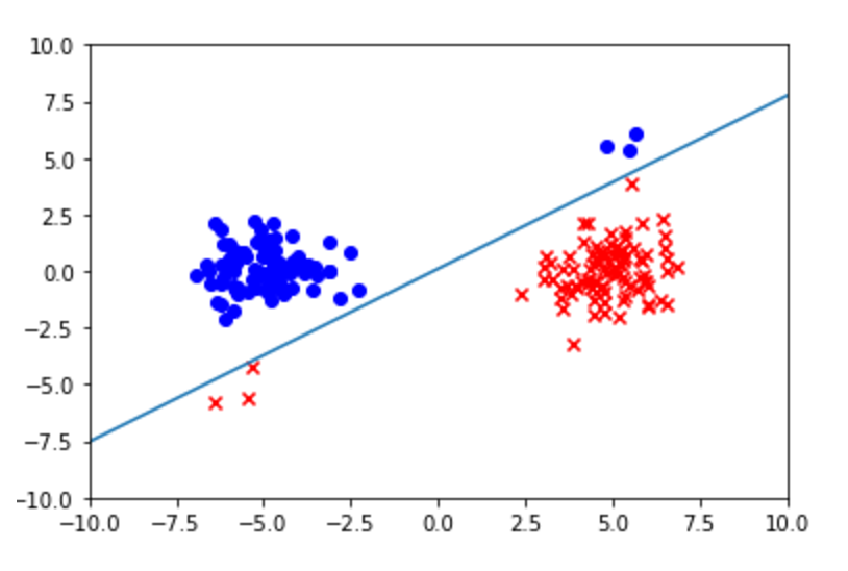
\includegraphics[width=0.6\textwidth]{figs/SVM_sample.eps}
  \end{center}
  \caption{SVMの直線による分類}
\end{figure}


\end{document}
